\documentclass[openany, a4paper]{book}

\usepackage{afterpage}
\usepackage{etoolbox}
\usepackage{fontspec}
\usepackage{geometry}
\usepackage{graphicx}
\usepackage{hyperref}
\usepackage{siunitx}
\usepackage{titling}

\newcommand*{\subtitle}[1]{\gdef\thesubtitle{#1}}

\title{CRAPS Kernel}
\subtitle{Final Report}
\author{
       Maxime Arthaud
  \and Korantin Auguste
  \and Martin Carton
  \and Étienne Lebrun
}

\newcommand{\risk}[4]{%
  \noindent
  \begin{center}
    \begin{tabular}{|p{0.8\textwidth}|c|}
        \hline
        #2 & $#1$
      \\\hline
        \multicolumn{2}{|p{0.9\textwidth}|}{#3}
      \\\hline
        \multicolumn{2}{|p{0.9\textwidth}|}{#4}
      \\\hline
    \end{tabular}
  \end{center}
}

\begin{document}
  \begin{titlepage}
  \begin{center}
    
\includegraphics[height=1cm]{LogoEnseeiht}\\\vspace{1cm}
    \hrule\vspace{0.5cm}
    \textsc{\Large\thesubtitle}
    \\\vspace{0.5cm}

    \textbf{\huge\thetitle}
    \\\vspace{0.4cm}
    \hrule\vspace{2cm}

    {\large
      Maxime~\textsc{Arthaud}      \\
      Korantin~\textsc{Auguste}    \\
      Martin~\textsc{Carton}       \\
      Étienne~\textsc{Lebrun}
    }

    \vfill
    {\large January -- March 2015}
  \end{center}
\end{titlepage}


  \chapter*{Acknowledgments}
    We would like to thank Jean-Christophe Buisson for giving us all the tools
    related to CRAPS that he has developed. We won a lot of time thanks to this.

    \paragraph{}
    We also would like to thank Bernard Desmyter and Benoit Lemarchand for
    having tested our compiler and showed us some bugs we did not see ourselves
    and Mickaël Carl for helping us with VHDL's best practices.

    \paragraph{}
    Finally, we would like to thank Xavier Mechin, our industrial supervisor,
    for guiding us throughout this two-month project.

  \tableofcontents

  \chapter{Introduction}
    \section{Context}
      This project, suggested by Daniel Hagimont, is based on the CRAPS
      processor developed by Jean-Christophe Buisson and used in the first-year
      Computer Architecture courses at ENSEEIHT. The goal is to develop an
      operating system that would run on top of that processor.

      Daniel Hagimont aims at doing an operating system course for ENSEEIHT
      students. The course would be based on the Computer Architecture course as
      Daniel Hagimont wants to add a more continuity in ENSEEIHT courses. At the
      beginning of the project it was only possible to do a little of assembly
      directly on the processor to see it working, but nothing more.
      After our project, it should be possible for students to really see
      the layer that goes on top of the CPU in modern computers: the operating
      system. Students should be able to really make the link between the
      processor and operating system they just built and the computer and
      underlying operating systems they use everyday.

    \section{Acronyms}
      \begin{description}
        \item[FPGA] A Field-Programmable Gate Array is an integrated circuit
          containing a lot of logic gates that can be programmed using a
          hardware description language such as \emph{VHDL}.
        \item[RAM] Random Access Memory is a kind of volatile memory were data
          and code is placed.
        \item[SHDL] Simple Hardware Description Language is the language used to
          implement the processor.
        \item[SPARC] Scalable Processor ARChitecture is a processor
          architecture.
        \item[VCS] Version Control System.
        \item[VHDL] VHSIC1 Hardware Description Language is the language
          \emph{SHDL} is compiled to. Some processor modules are written
          directly in \emph{VHDL}.
      \end{description}

    \section{Pre-existing code and tools}
      \emph{CRAPS} is a simple processor conceived by Jean-Christophe Buisson
      for the first year Compiler Architecture course. It is inspired from the
      \emph{SPARC} architecture. It is written in \emph{SHDL}, a simple hardware
      description language also developed by Mr.\ Buisson.

      The processor is loaded on a Spartan-3E \emph{FPGA} (see
      figure~\ref{fig:nexys}).

      \begin{figure}[h]
        \centering
        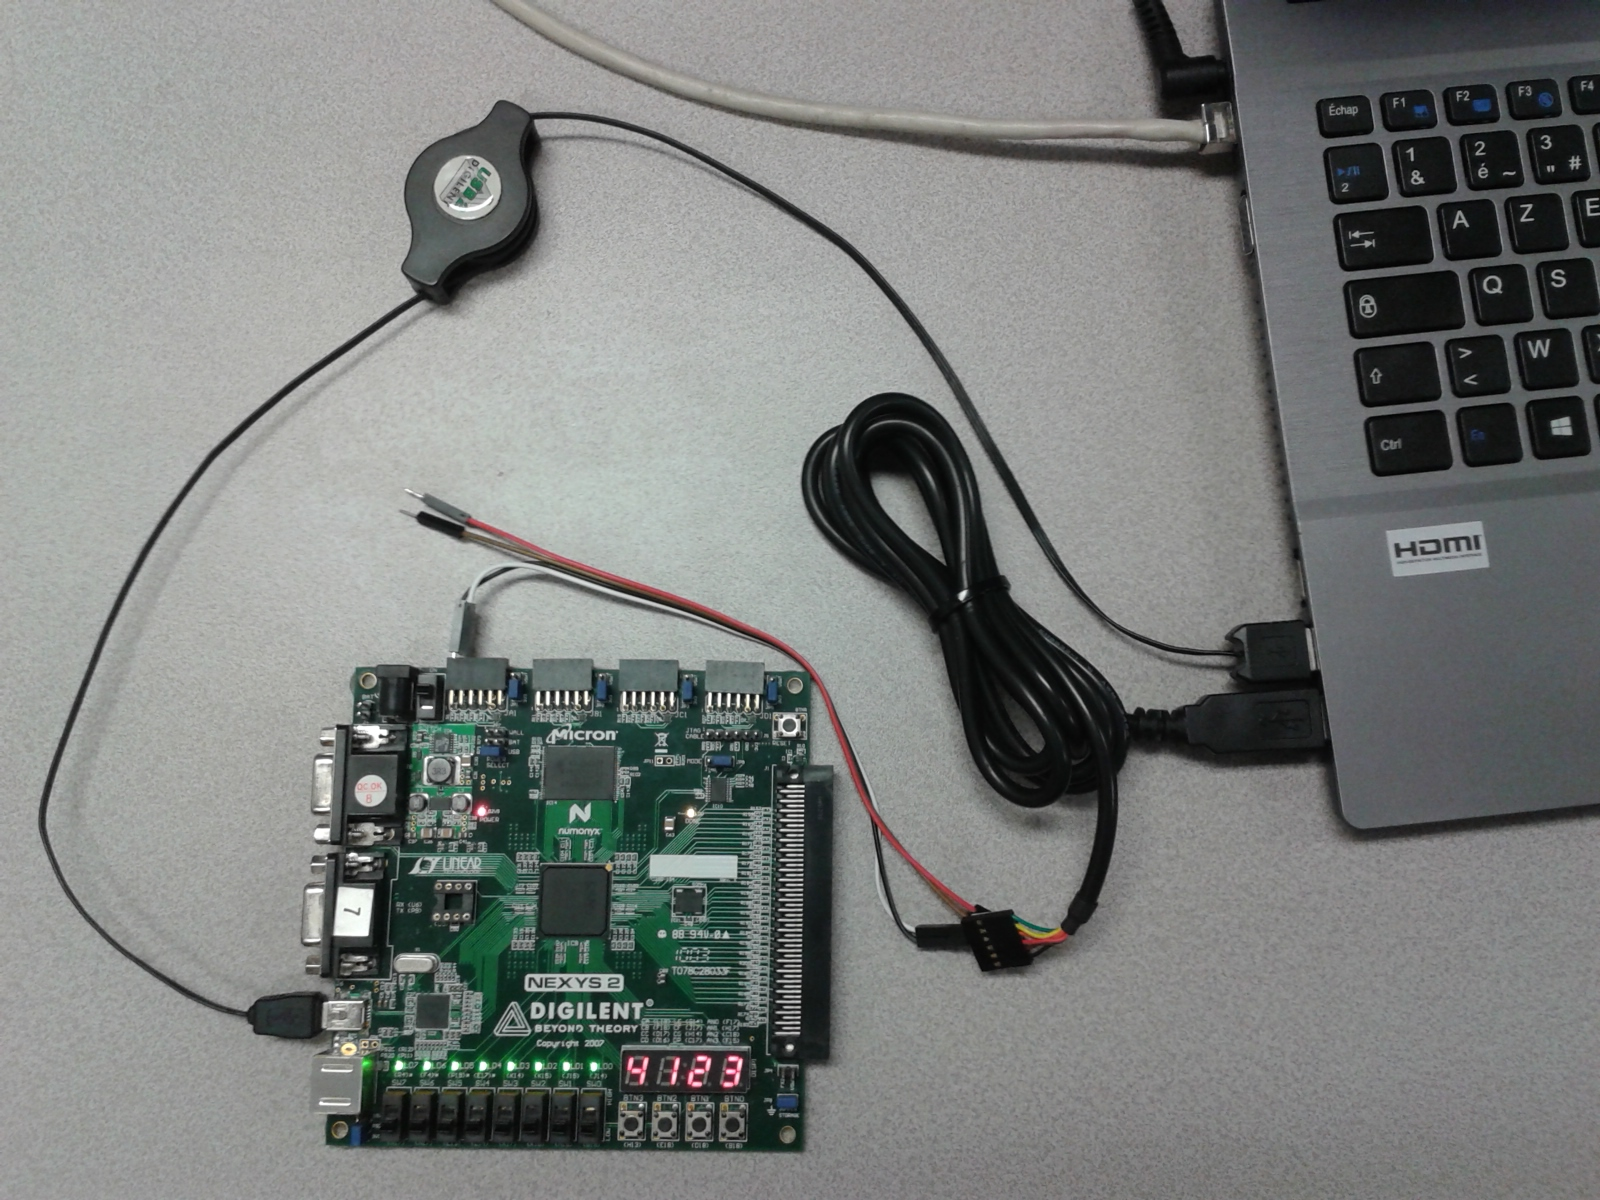
\includegraphics[width=0.8\textwidth]{./fig/Nexys2.jpg}
        \caption{A Nexys2 board}
        \label{fig:nexys}
      \end{figure}

      In the beginning of the project, we were given:
      \begin{itemize}
        \item the \emph{SHDL} source code for the CRAPS processor;
        \item the source code for the \emph{SHDL} compiler: it takes \emph{SHDL}
          code, produces \emph{VHDL} code and uses an external tool to
          synthesise the design and create the final file that can be loaded on
          the \emph{FPGA};
        \item the source code for the monitor that interacts with the processor
          on the board and contains the assembler to generate \emph{CRAPS}
          bytecode from the \emph{CRAPS} assembly code.
      \end{itemize}

    \section{Work required}
      The project is composed of three main tasks:
      \begin{itemize}
        \item improve the simple processor developed by students to add missing
          features;
        \item create a compiler for a \textit{C-like} language to the
          \emph{CRAPS} assembly language;
        \item the operating kernel system itself.
      \end{itemize}

      All tools and source code produced will need to be documented for both
      teachers and students.

    \section{Available resources}
      Jean-Christophe Buisson initially lent us 2 boards. As this was not enough
      for the four of us to work efficiently, he lent us 4 more boards.

      Our client got us a room in ENSEEIHT to work.

      \paragraph{}
      We also set up a \textit{git}\footnote{\textit{git} is a distributed
      VCS.} repository to put all the sources and
      document we have produced during this project. This allowed us to
      efficiently work simultaneously on the same files and keep a history of
      all changes.  We also set up a mailing list and a Jabber
      room\footnote{\textit{Jabber} is an instant messaging protocol.} to
      communicate with each other.

      We did all the work on our own personal computers.

  \chapter{Project management}
    The team is composed of four members:
    \begin{itemize}
      \item Korantin Auguste as \textit{developer}
      \item Maxime Arthaud as \textit{tester}
      \item Martin Carton as \textit{project leader}
      \item Étienne Lebrun as \textit{quality manager}
    \end{itemize}

    We were initially 5 but one of us had to leave the team for medical reasons
    at the beginning of the project.
    The fact that we know each other and have already worked together on several
    occasions made the management easier, and we did not need a very strict
    repartition of the tasks.

    \section{Project supervision}
      We were affected to Xavier Mechin, quality control manager at Airbus
      Defence and Space to guide us in managing our project. Martin and Maxime
      met him the week before the project started (Korantin and Étienne were
      abroad). We decided to meet once a week. The date and order of the reunion
      is as follow:

      \begin{itemize}
        \item Week 0 (January 15th): presentations;
        \item Week 1 (January 22th): presentation of all members, presentation
          of the project management related work to do;
        \item Week 2 (January 28th): first review of the software development
          plan and specifications;
        \item Week 3 (February 4th): canceled due to the weather conditions;
        \item Week 4 (February 10th): review of the software development plan
          and specifications;
        \item Week 5 (February 18th): planning of the testing phase;
        \item Week 6 (February 25th): review of the test plan, planning of the
          final report and presentation;
        \item Week 7 (March 4th): review of the draft of final report;
        \item Week 8 (March 10th): review of the final report and draft of
          slides for the final presentation.
      \end{itemize}

      During these meetings, Xavier explained us what documents we should
      produce for the management of the project and how to use them. Of course,
      as our project was short, we did not follow all Airbus practices but this
      showed us how do companies such as Airbus manage their projects.

      \section{Planning and distribution of tasks}
        Once the work on the specifications was advanced enough (cf.\ 
        section~\ref{sec:spec}), we gave a rough time estimate for each
        task, and took into account finish-to-start constraints to make a
        planning (see figure~\ref{fig:gantt}). Each one decided what he wanted
        to work on.

        When someone encountered difficulties (which happened in particular for
        the RS-232 and the flash), he could ask for help, and another member of
        the team would come to help working on his task.

        We updated the planning each week, with approximations of the
        advancement on each task. It was quite difficult to estimate how long
        would each task take, but at the end the planning was a great help to
        know what was done, what was to be done and if we were late.

      \section{Risks management}
        In order for the project to be as smooth as possible, we made a list
        the events that could threaten the project, and defined actions to
        limit the risk. We were able to identify three risks.

        For each risk, the product $\text{probability} \times \text{gravity}$ is
        shown in the top-right cell. If the product is above 6, the risk is
        considered critical.

        \risk{3 \times 3 = 9}{
          A \emph{FPGA} can be damaged, making any test impossible.
        }{
          This is likely to happen and very problematic but we have two
          \emph{FPGA}s and the possibility to have more in case of problem.
        }{
          Actually, we have 6 \emph{FPGA}s, the risk is considered closed.
        }

        \risk{2 \times 3 = 6}{
          We may not be able to integrate the RAM, leading to huge memory
          limitations that may make the project impossible.
        }{
          We are now able to use the RAM, the risk is closed.
        }{
          In case of memory limitations, we can try to optimize the size of the
          code we generate.
        }

        \risk{3 \times 1 = 3}{
          The communication between the board and the computer might be too
          slow.
        }{
          We will have to be very careful to send just what is needed.
        }{
          We would need to limit the communication. It is not necessarily a
          problem as this is just to show students how to implement a simple
          communication protocol.
        }

        It was a bit difficult at first to identify the risks, but these three
        were very pertinent.

        The first risk was put in evidence by Mr.\ Buisson, who told us that
        some specific misuse of the card could lead to permanent damage. We
        managed not to damage any board.

        The second risk was a big concern during a big part of the project, as
        it was difficult to integrate the RAM. We worked on reducing the size of
        the generated code, but at the end of the project, it was even possible
        to map the external RAM chip (but it was considerably slower).

        The third risk was not solved, however if we communicate slowly enough
        from the computer, everything works fine. We don't think the impact of
        that problem is very important as the main goal of the communication
        (make a small shell on the board) is implemented and works properly at
        that speed.

    \section{Actions Management}
    Our actions file takes the form of a spreadsheet (see annexe
    \ref{ActionFile}). On this file, we listed the actions we had to do. Each
    action has a description, the event that caused it and the date of cloture.
    We mainly used it to distribute the redaction of minutes among us. We also
    kept track of some other actions related to the technical aspects and
    exceptionnal events.

  \chapter{Specification phase}
    We planned a meeting with the client the first day of the project. He
    explained us what he wanted us to do and that the project was very flexible.
    His goal is to be able to make lab sessions for first-year students of
    ENSEEIHT. Thus, as long as he can show students how an operating system
    works the project will be a success.

    \section{Redaction of the technical specifications}\label{sec:spec}
      Once we had determined the client's needs, we had to specify exactly what
      we had to do. This phase was difficult as the client was imprecise about
      what we had to do. We decided to do split the project in three distinct
      steps:
      \begin{itemize}
        \item in a first time, develop the tools to write the  most basic
            functionalities;
        \item then add a possibility to communicate with the OS with through the
          serial port;
        \item finally, be able to load and run program dynamically.
      \end{itemize}
      Once these steps were decided, we refined them into several tasks that
      could be done by the different members of the group.
      Each requirement is numbered in the specification document.

    \section{Technical choices}
      We choose to work as much as possible on GNU/Linux as this is our
      daily-use operating system and the operating system installed on most
      ENSEEIHT computers.
      However, some tools we needed were designed to work exclusively on
      Microsoft Windows. To get around this problem, we decided to use the
      Windows-specific tools in a virtual machine or adapt tools to GNU/Linux
      when possible. We ended up adapting the monitor, and using it as a basis,
      we wrote a distinct compiler tool (\verb+crapsc+) to generate the
      bytecode, and a command line debugger, \verb+crapsdb+. We decided not to
      bother adapting the tools to synthesise the processor, and keep using them
      on the Microsoft Windows virtual machine.

      \subsection{Compiler}
        We had to write a compiler but as this is a very time-consuming task, we
        decided to reuse the compiler we had to write for a previous ENSEEIHT
        project. This compiler did not target the CRAPS machine, but we made it
        modular enough to able to easily add a CRAPS back-end.

        We considered for a moment to write a CRAPS back-end for
        \emph{LLVM}\footnote{\emph{LLVM} is a compiler infrastructure
        offering a set of reusable libraries, it gives a way to write specific
        backends.\cite{llvm}}. This would have had the advantage to be able to
        use \emph{clang}, a real, complete and optimized \emph{C} compiler. But
        the work it would have required seemed to be too important as we did
        not know the \emph{LLVM} infrastructure and the infrastructure contains
        a lot of features we would not have used but would have had to
        support.

        \paragraph{}
        Finally, this was a good choice: The compiler we have made is really
        complete and even able to make some optimizations.

        We have extended it we made to accept a language closer to \emph{C} and
        have added a lot of missing features. We also take some time to improve
        the generated code to use as few memory as possible as the target
        machine is quite limited.

  \chapter{Implementation phase}
    \section{Hardware extension}
        In order to write an OS, we needed to extend the micromachine.
        It lacked several key elements:
        \begin{itemize}
            \item the possibility to handle several interrupts
            \item enough RAM to load a program the size of the kernel.
            \item serial port communication
        \end{itemize}
        \subsection{interrupts}
            To handle interrupts, we added a module. It registers when its
            inputs are activated and returns the interrupt of higher level.
            Another input is activated when the higher interrupt has been
            treated.
        \subsection{Block Ram}
            The first version of CRAPS had only 512 words of memory. This
            memory was asynchronous, which prevented the synthesizer from
            mapping it in the dedicated block RAM of the FPGA. Using a
            synchronous implementation, we were able to access the block RAM,
            and integrate up to 48K bytes of memory in the processor. This 
            however caused timing issues. The block ram can not be read directly
            and a little amount of time is needed for the value to be put in a
            reading buffer. We chose an easy way to deal with this problem, 
            adding a waiting cycle in the sequencer. 
        \subsection{Flash memory}
            We thought that it would be interesting to use the persistent memory
            that is available on the board to create a little file system, and 
            store user programs. We spent a lot time figuring out how to
            communicate with it, based both on the memory chip specifications
            and the digilent implementation of a module that accesses the flash
            memory. This still did not work. We finally realised that the issue 
            was that we had to erase a block before writing it. This meant that
            we could not use the memory as we intended to, and we abandoned this
            idea.

        \subsection{External RAM}
            As the flash and the RAM share an interface and handle in a similar
            way, the work done for the former could be adapted to use the
            external ram module. A bit more work was required to interface it
            nicely with the processor, and be able to only manipulate 32 bit
            words(which means we can directly use it to store programs if
            needed). 
    \section{Description of the interrupts}
      We first had to develop an interrupt system to have the possibility of
      executing code when receiving some events. When an interrupt is triggered,
      the current task pauses to let the interrupt handler execute. This needs
      to be completely transparent for the task.

      \subsection{PWM interrupt}
        This is the first interrupt we have integrated. The PWM interrupt is
        triggered at regular interval and gives us the possibility to write the
        scheduler (see section\ref{sec:scheduler}).

      \subsection{Buttons interrupt}
        We have created a specific interrupt for each of the three available
        buttons on the board. This is not of any useful use anymore but it was
        very handy during the development of the interrupt handler as it allows
        humans to directly interact with the board.

      \subsection{RS-232 interrupt}
        We had to add a specific interrupt for the serial port communication.
        An interrupt is triggered whenever a byte is received. The corresponding
        handler caches this byte in a buffer. It has to be fast as the byte
        is removed from the \emph{VHDL} module when we receive the next byte.

        Another interrupt handler should be triggered when the serial port is
        ready to send a byte but it does not work. When we try to use the
        corresponding bit in the VHDL module, the processor freezes. We did not
        resolve this problem as we have no idea of what causes it.

      \subsection{Software interrupt}
        The higher level interrupt is not triggered by the hardware, but is
        used to implement system calls. A program can access system functions
        such as memory management by putting their argument on the stack and
        calling a special assembly instruction. This instruction creates an
        interrupt, which is handled by the operating system. It will check the
        first value on the stack, which indicates what system function was
        called, and then launches the corresponding function. The fact that this
        is the higher level interrupt makes it not interruptible, which allows
        us not to worry about concurrency.
    \section{Scheduler}\label{sec:scheduler}
      The scheduler is the component that makes it possible to execute more than
      one task at a time: It will switch between all running task in a very fast
      way, giving the illusion that all processes runs at the same time.

      To make it work, we had to create a specific interrupt that will be
      triggered regularly by a clock. This interrupt saves the execution
      context (all the registers and flags of the processor) and restores the
      one of the next process to execute. The process must be completely
      transparent, as a task should not be distributed by a context switch.

      To do that, we also have a data structure containing the list of the
      processes. First, it was simply a list resized when we added or deleted
      processes. However, we ended up changing it to a list of a fixed size,
      containing either a pointer to processes stacks, or a null value.
      This allowed the processes to have a fixed ID that will not change during
      their life. With that knowledge, the process management was made
      easier, and it was also possible to annotate memory zones with the
      associated process ID, leading to clean freeing of all the memory
      allocated by processes when they were terminated.

    \section{Serial Port}
      In order to communicate with the OS from another device, we added a UART
      (Universal Asynchronous Receiver Transmitter) module. We used the RS-232
      reference module available on the Digilent website. The most difficult
      part was actually to modify the \emph{SHDL} to \emph{VHDL} compiler to add
      a predefined \emph{VHDL} module, directly accessible from the \emph{SHDL}.

      Due to hardware limitations, the communication is rather slow. Each byte
      is transmitted with a baud rate of 9600, but we still have to wait
      between each byte.

      \subsection{OS implantation}
        When a byte is received, an interrupt is triggered. The handler
        reads the byte from the UART and puts it in a circular buffer.
        Processes that want to receive data read from this buffer. Processes can
        also write directly to the UART to send a byte.

        It would be nice to make the communication through system calls. It
        would allow us to implement communication canals, which would allow
        several processes to use the serial port simultaneously.

    \section{Memory management}
      For the dynamic loading of processes to work, we needed to be able to
      allocate memory zones (for processes stacks). It was also really important
      to have the possibility for processes to allocate the memory they need.

      Thus we had to create the equivalent of \verb+malloc+, \verb+realloc+ and
      \verb+free+. We did a very
      simple implementation: starting from a base pointer, we store block of
      memory. These blocks start with a header indicating their size, the
      process ID that allocated them (and a byte to tell if the block is free or
      not).

      The size of each block is a power of two. So when we allocate a block, we
      will try to see if there is a free block of the good size. If there is
      not, we will create a new block at the end of the block list.
      So, we don't merge or split blocks, and will waste memory. But it keeps
      the implementation simple, and in general the block are reused a lot.

    \section{Compiler}
      We needed to support a language very close to \textit{C} that could be
      compiled to \emph{CRAPS} assembly.
      A document that summarize what language constructs are available and the
      differences with real \textit{C }has been written as part of the
      documentation.

      \subsection{Optimizations}
        We worked on some optimizations for the compiler. Our main goal was to
        minimize the size of the generated assembly.

        The compiler is now able to remove unused functions. It is also able to
        simplify arithmetics expressions and compute addresses at compile-time.
        It uses as much as possible registers with a fixed value (such as
        \verb+%r0+ and \verb+%r20+), and uses optimized instructions like
        \verb+sethi+ or\verb+setq+.

        We also added the \verb+register+ keyword that allows a variable to
        be stored in a register. Variables stored in registers are much faster
        than the ones in memory.

        After a benchmark, we concluded that the optimizations made reduces the
        size of the generated assembly by approximately $25\%$.

      \subsection{Position Independent Code}
        The compiler has to generate Position Independent Code as we need to be
        able to dynamically load code. This required to make some modifications
        to the compiler.

        It also required to set a new convention for a register to hold the
        value of the global data section of the current code.

    \section{Dynamic loading}
      One of the last task we had to make was to make it possible to
      dynamically load code on the board, and run it.

      This was implemented on our "shell" task, as we made a new command that
      will receive code transferred by the serial, in a newly allocated
      memory zone.  Then, a stack for the new process will be created and the
      process will be ran.

      The biggest problem was to have fully position-independent code (when
      we compile code, it references variables that are at absolute addresses
      in memory, and the code can be loaded at any address). To solve that
      problem we defined a register, \verb+%r24+, that contains the address of
      static data so all the references are relative to this base address.

      The memory layout of the kernel is presented in figure~\ref{fig:memory}.

    \section{Final result}
      Our final result is a micro "operating system" running on the board.

      By default, it runs a task called the shell, that will receive command by
      the serial port.  So, we can then connect the board to a computer, and
      send command to the board.

      Among these command, it is possible to list the active process, and start
      built-in tasks (a counter, a task to control the LEDs on the board \dots).
      We can also load code that was compiled on the computer using dynamic
      loading. We can also kill running processes.

      \subsection{Example of use}
        TODO: Add screens of the shell (real screens of a terminal), and list
        commands.

  \chapter{Validation phase}
    \section{Tests}
      The tests were not easy to do. We tried to automate them as much as
      possible, unfortunately, it was not always possible.

      The tests for the three main tasks are independent, but as the kernel
      obviously use the compiler and the processor, the tests for these two
      tasks were really important.

      \subsection{Processor}
        The individual components of the initial version of the processor had
        already been tested, so we did not test them more thoroughly. Some test
        programs had also been written, and we made sure that our processor
        still passed them after we modified the sequencer.
        The tests for the hardware modules written in VHDL could not be
        automated, as they require a special environment which was too long to
        set up properly, given the short time we had at our disposal.

        Once the new modules had been integrated in the processor, we wrote
        test programs to validate that they were working properly. These have
        to be done manually, as they require to check values in register or to
        look at the seven segments display. These tests were written directly in
        assembly code, in order to dissociate eventual errors of the compiler.

      \subsection{Compiler}
        The compiler has two kinds of tests.

        The first tests are fully automated and tests if the compiler succeeds
        to compile valid program and fails to compile invalid programs. We have
        plenty of such tests and we tried to be as exhaustive as possible. They
        do not test the compiler correctness.

        The other kind test if the compiler generates valid code. These tests
        are not automated as we need to upload the code on the board after the
        compilation. Most of these tests are expected to produce a specific
        output on the 7-segment display when then succeed.

      \subsection{Kernel}
        We have made less tests for the kernel itself, as the only way we had
        to test it was to make sure that the programs we wrote were executed
        properly.

        We tested independently the main components such as the scheduler and
        the memory allocation functions and validated them.

        What serve as a good test is the use case we designed for our client. We
        were able to realise a series of actions (such as loading program
        dynamically and launch them) without the kernel showing unexpected
        behaviour.

        And of course, for both the processor and compiler, the ability to run
        the kernel is the ultimate test.

    \section{Limitations}
      The project has some limitations:
      \begin{itemize}
        \item The communication is quite slow, but sufficient for a shell.
        \item We were not able to use the flash memory. As such, the board
          has no persistent memory.
      \end{itemize}
        The project is however a success, even if we wish we had had time to
        incorporate even more features. It would indeed have been nice to have a
        file system, or even VGA communication support.

  \chapter{Conclusion}
    Despite the difficulty and the amount of work brought by this project, it
    was a great and exciting experience. First we learned the bases of project
    management, field we were not familiar with because of the shortness of our
    previous ones. Moreover, the width of explored technologies made this one
    particularly fascinating and its realisation an achievement. Finally,
    developping on CRAPS, the very processor we built in our first year at
    ENSEEIHT made us kind of nostalgic and realising all the progress we made
    throught all of this wonderful years. Thus we hope that future students will
    be as pasionate as we were and that the moc language will shine over the
    years.

    That's why we proudly consider this project as a success.

    % This was a passionating project and we think it was a success. The client
    % seems to be very happy with our work, we really hope he will be able to use
    % our work in his classes and that ENSEEIHT students will be as passionate as
    % we were to do this project.

    % The project was a good occasion to learn how to manage a project, which we
    % never really needed for our previous projects as there were too short.

  % reset the chapter counter and use lettered-chapter from now on
  \setcounter{chapter}{0}
  \renewcommand{\thechapter}{\Alph{chapter}}

  \patchcmd{\thebibliography}{\chapter*}{\chapter}{}{}
  \begin{thebibliography}{9}
    \bibitem{buisson}
      Jean-Christophe Buisson,
      \emph{Introduction à l'architecture des ordinateurs},
      Chapitre VII.\ CRAPS~: guide du programmeur.

      \mbox{\url{http://diabeto.enseeiht.fr/download/archi/cours/book2_4.4.pdf}}

    \bibitem{nexys2}
      \emph{Digilent Nexys2 Board, Reference Manual},
      Revision: July 11, 2011.

      \mbox{\url{http://www.digilentinc.com/data/products/nexys2/nexys2_rm.pdf}}

    \bibitem{llvm}
      \emph{Writing an LLVM Backend}

      \mbox{\url{http://llvm.org/docs/WritingAnLLVMBackend.html}}
  \end{thebibliography}

  \chapter{Annexes}
    \newgeometry{left=1cm, right=1cm, bottom=1cm}
    \begin{figure}
      \centering
      \includegraphics[height=0.9\textheight]{build/memory_layout_fromsvg.pdf}
      \caption{Memory layout of the kernel}\label{fig:memory}
    \end{figure}

    \begin{figure}
      \centering
      \includegraphics[height=\textwidth, width=\textwidth, keepaspectratio]
                      {build/micromachine_old_fromsvg.pdf}
      \caption{Old version of the CRAPS micromachine}
    \end{figure}

    \begin{figure}
      \centering
      \includegraphics[height=\textwidth, width=\textwidth, keepaspectratio]
                      {build/micromachine_updated_fromsvg.pdf}
      \caption{Updated version of the CRAPS micromachine}
    \end{figure}

    \begin{figure}
      \centering
      \includegraphics[height=\textheight, width=\textwidth, keepaspectratio]
                      {Gantt.pdf}
      \caption{Last version of the Gantt diagram}\label{fig:gantt}
    \end{figure}

    \begin{figure}
        \centering
        \includegraphics[height=\textheight, width=\textwidth, keepaspectratio]
                      {Actions/ActionManagement.pdf}
        \caption{Our Actions file}\label{ActionFile}
    \end{figure}

\end{document}
